\section{Software Design}
\phantomsection

\subsection{UML Modeling}
In the current chapter is represented and described the architecture of DSLR Camera Controller application. It contains a set of relevant diagrams modeled in UML language. The diagrams provide a fundamental documentation an description of the system structure and behavior.

The aspect that should be defined is how the user will interact with the application. Therefore a use case diagram was modeled to show the set of available actions offered at the user's disposal. The client part of the application represents a browser web page. There are six main actions a user can perform. The operations can be seen in \mbox{figure \ref{use_case}}. When the application is opened, the user can view/manage the connected cameras. The seconds main action is to manage a selected camera's settings. The app should detect all available configurations supported by the camera, if it has any. Next, the user can take a photo and get a live preview as well. Additionally, the user is allowed to configure a failure strategy. And finally, the main action is to allow the user to configure a time-lapse.

\begin{figure}[!ht]
\centering
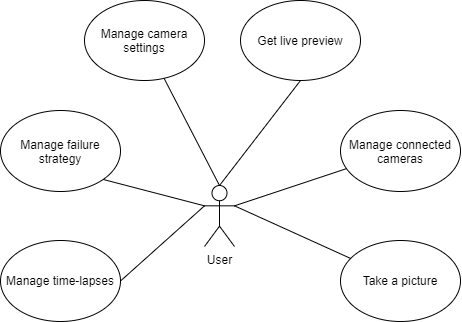
\includegraphics[width=15cm]{2-user-use-case-diagram}
\caption{User use case diagram}\label{use_case}
\end{figure}

To offer a detailed overview of how the entire system works, a set of sequence diagrams are provided. They show key parts of the platform and the way they interact. Moreover it is crucial to depict the depth of chain of events happening in the background. For instance the sequence diagram, shown in \mbox{figure \ref{user_sequence}}, specifies what happens when a user simply asks for camera settings. First of all the client browser does an HTTP request in order to get the application page. Now the user is able to interact with the platform. When the client requests the settings on a detected camera, the application first has to ask the selected camera's available configurations. The camera, if it supports this feature, will return a list of settings. These settings also include read-only configurations, like serial number or camera power, so the application filters the known read-only configurations and returns them to the user.

\begin{figure}[!ht]
\centering
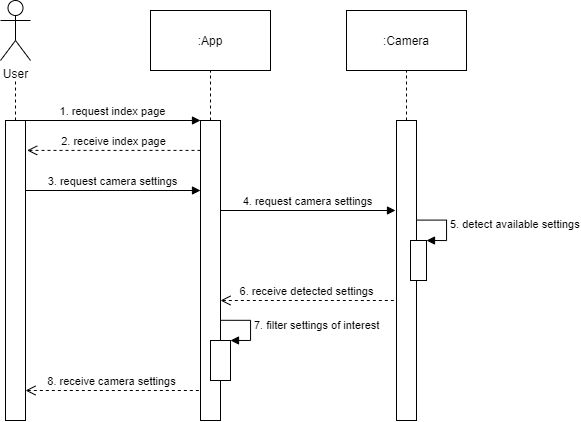
\includegraphics[width=15cm]{2-user-sequence-diagram-get-cam-settings}
\caption{Camera settings sequence diagram}\label{user_sequence}
\end{figure}

For time-lapses we can distinguish two main steps. Each one is described in the sequence diagrams illustrated below. Their behavior looks a bit similar, nevertheless each has unique characteristics worth point out.

The first step of a time-lapse is the process of scheduling one, that is depicted in \mbox{figure \ref{timelapse_request_sequence}}. First, the user requests a new schedule. The most important data that the user has to provide is the \textbf{cron} expression, which is used for scheduling. The request is then processed in the application, so that it is configured to require the currently connected cameras. If a camera is missing during a capture event, the platform will consider it as a failure and will take the appropriate measures (send email notifications, hard reset, etc.). Next, a special worker that runs separately from the main thread receives the request. The worker then registers the new time-lapse into a persistence mechanism and computes its next run based on all available time-lapses. Reading all the active time-lapses from the database is not the most optimal method, but considering that there will usually be only one active time-lapse, it can be considered satisfactory. At the end, the user receives a success message with the newly created schedule.

\begin{figure}[!ht]
\centering
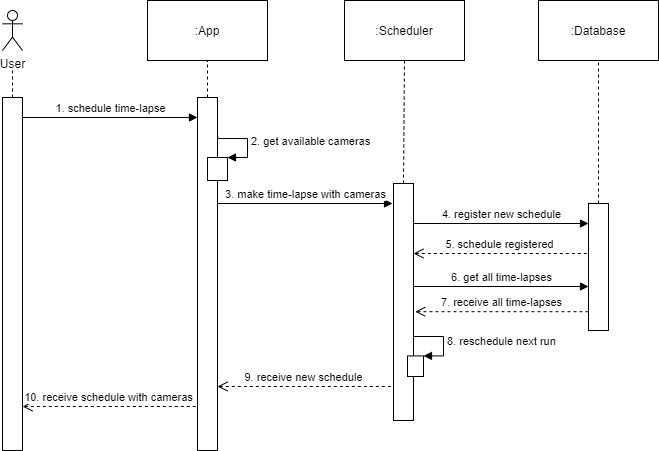
\includegraphics[width=15cm]{2-timelapse-request-sequance-diagram}
\caption{Time-lapse requesting sequence diagram}\label{timelapse_request_sequence}
\end{figure}

The sequence diagram, illustrated in \mbox{figure \ref{timelapse_triger_sequence}}, represents the next step after the user has successfully registered a time-lapse. When the Scheduler triggers a capture event it runs an abstract command composed by the application. This command goes through the list of required cameras and tries to take a picture. After the picture was taken, the scheduler recomputes when it should run the next time. Afterwards, an event that the picture was successfully taken is then published. The application has a special handler for this event which transfers the file if it was configured to do so, then it logs the successful capture and transfer.

\begin{figure}[!ht]
\centering
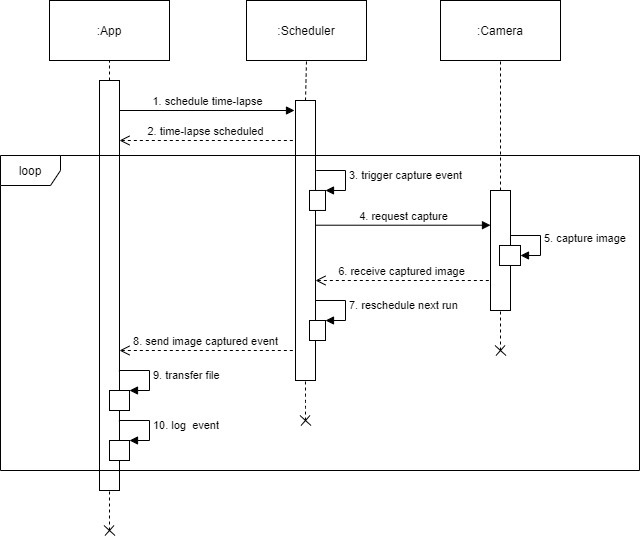
\includegraphics[width=15cm]{2-timelapse-triger-sequance-diagram}
\caption{Schedule capture trigger sequence diagram}\label{timelapse_triger_sequence}
\end{figure}

The time-lapse is the most crucial feature of the application. So, to better understand how it works, in the figure \mbox{\ref{timelapse_iteration_activity}} is described through an Activity Diagram a single iteration of the time-lapse. It starts by rescheduling its next run. When a capture event is published, the application requests the time-lapse's cameras to take a picture. If a camera is missing, or one of the cameras returned an error, or some error happened, the application registers it as an error. The details of the failure are registered in a special logging system that the user can later query from the web. Afterwards the failure process starts. Otherwise, if there were no errors while taking photos, the photo is logged and then the file transfer routine starts, independent of photo capturing routines. Again, if an error occurs in this step, it is also logged in the system.

\begin{figure}[!ht]
\centering
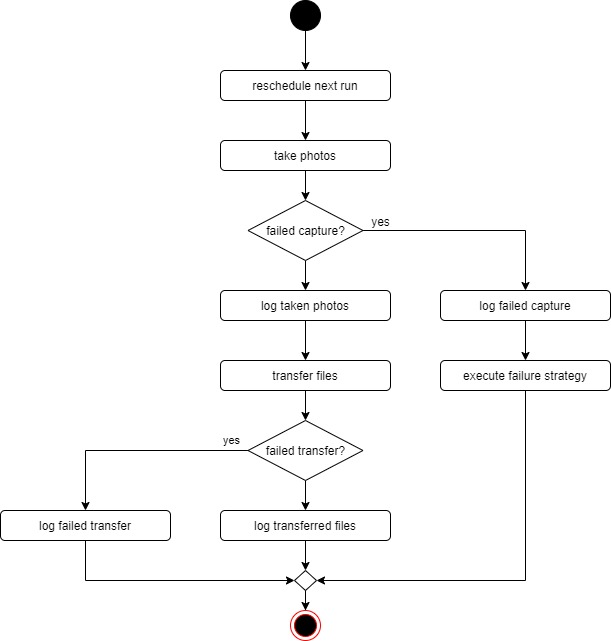
\includegraphics[width=14cm]{2-time-lapse-iteration}
\caption{Time-lapse iteration activity diagram}\label{timelapse_iteration_activity}
\end{figure}

The processing of the capture failures is a key feature of this application as well. Coming up with a few practical solutions that would work across multiple camera models was not an easy task. Nevertheless, in the figure \mbox{\ref{timelapse_failure_activity}} is described the activity diagram of how the failures are being handled. This is an extension of the diagram from the figure \mbox{\ref{timelapse_iteration_activity}}. First, if the user has enabled the email notification feature, on failure, the application will fetch all the emails registered for notifications and send them the error message. Then, if hard resetting is enabled, the application will first try to programmatically reconnect to the cameras. In some cases this is good enough, as some camera models simply require a wake-up call. Then, if an Ykush device is detected to be connected to the system, then it activates it as well, which basically re-plugs the cameras. Re-plugging almost always solves any problems it might have encountered. And finally, if system rebooting is enabled, the program will reboot the system after a consecutive number of failures. This allows the user to reset the USB connections at the expense of processing time. But considering that it is cheaper than an external device for reconnecting the USB connections, this may be viable enough option as well.

\begin{figure}[!ht]
\centering
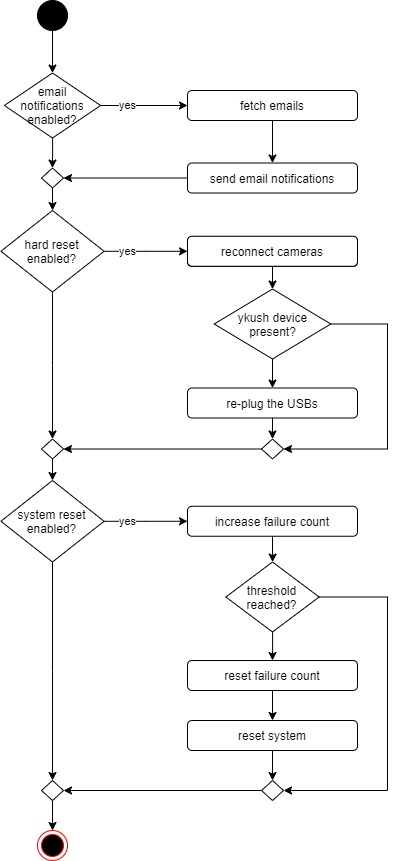
\includegraphics[width=7cm]{2-timelapse-failure-activity}
\caption{Time-lapse failure activity diagram}\label{timelapse_failure_activity}
\end{figure}

In the following part of this chapter is described the most important classes of the DSLR Camera Controller application through a few class diagrams. Most of them are related to the camera and time-lapse management. Information about the system components interaction is not enough for understanding the tool. The class diagrams deliver information under a higher level of granularity, hence the system becomes more easy to comprehend.

First in the figure \mbox{\ref{camera_manager_class_diagram}} is described how the application is using the cameras. The concept of camera is completely abstracted from the core. The whole application simply communicates with an abstract camera that is known to have a few functionalities like capturing an image, setting a configuration, etc.. Binding the application to the fact that the cameras are connected through some ports or that it is using a special library to communicate with the camera would transform the maintenance of the application into a nightmare. That's why the implementation of the abstract camera and camera manager sits in the infrastructure level of the application. To allow testing of some functionalities without any cameras connected, some fake cameras were introduced with a few predefined configurations like output image, available setting, etc.. CameraManager works with cameras, but the implementations are aware what kind of cameras they are working with, so it is not quite the Bridge design pattern implemented here.

\begin{figure}[!ht]
\centering
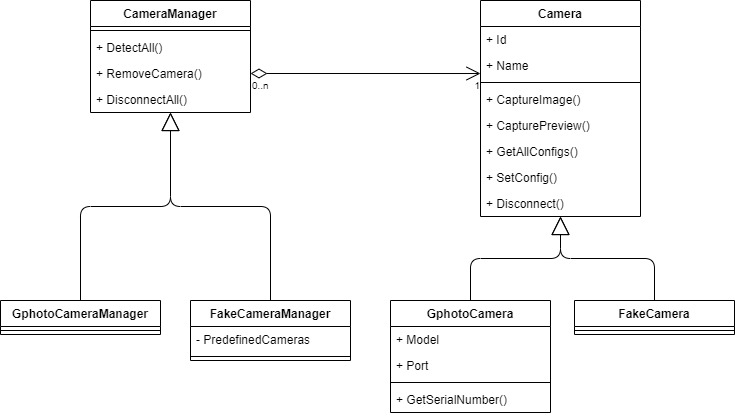
\includegraphics[width=18cm]{2-camera-manager-class-diagram}
\caption{Camera management class diagram}\label{camera_manager_class_diagram}
\end{figure}

Next follows a class diagram on how a time-lapse is persisted on the platform. In the figure \mbox{\ref{timelapse_data_class_diagram}} is represented what data is required for a time-lapse. It is composed of a nullable schedule and has reference to the required cameras. If the schedule is null, then it means that the time-lapse has been put on hold. The separation of the time-lapse from the schedule offers the possibility to reuse the scheduling logic for other features. One of the requested feature was to email a monthly report on the progress of the application.

\begin{figure}[!ht]
\centering
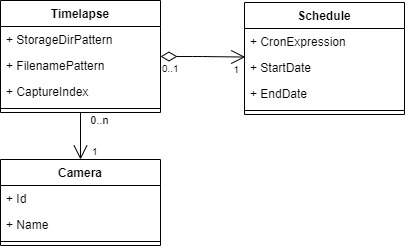
\includegraphics[width=13cm]{2-timelapse-data-class-diagram}
\caption{Time-lapse data class diagram}\label{timelapse_data_class_diagram}
\end{figure}


% The platform modules and their behavior were described until now. Another important part of the application is the set of libraries it uses and their purpose, depicted in \mbox{figure \ref{component_diagram}}. Because the project is divided in two parts there are two set of dependencies and libraries. The data mining part is a console applications, hence the set of required libraries is small. The essential library is rest\_client, used for requesting web pages and getting their content. Nokogiri is used for parsing HTML and extracting the necessary elements. Savon is a library for SOAP communications, needed for NLP processing. Mongoid is used for database communication, as it was discussed above. The client part of application requires more libraries because it consists from more logical components. Some gems (a ruby term for library) are shared between the logical components, for example Mongoid. Sinatra framework is used to build the web applications. The main goal is to handle client's HTTP requests. Faye library is used to host the websocket server. It is handy because it provides a higher level of functionality than a simple websocket. Haml gem aims to process the haml files for creating web page content. Haml is a dialect of HTML, simply put another markup language. Sidekiq is a library used for running asynchronous jobs. Redis is a dependency required by Sidekiq and it is used as a message queue system. D3 is a JavaScript library used for drawing plots and charts. This sums it up. Of cores there are also other dependency libraries.

% \begin{figure}[!h]
% \centering
% 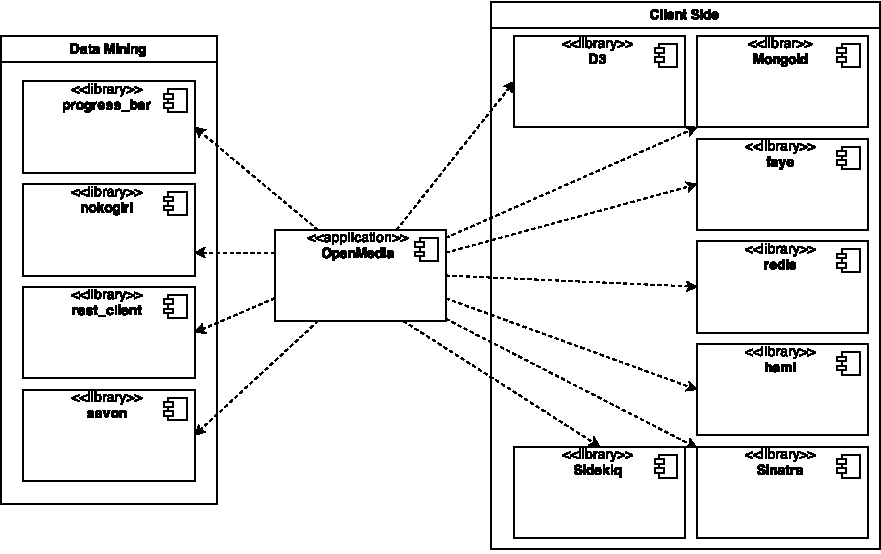
\includegraphics[width=16cm]{2_component_diagram}
% \caption{Component diagram of OpenMedia}\label{component_diagram}
% \end{figure}

% The deployment diagram gives a good understanding of the whole system. OpenMedia platform has a complex structure and consist of more than a few modules, see \mbox{figure \ref{deployment}}. In order to launch the application, not every module needs to be up and running. Data mining application is a console ruby applications which only requires to run once in a while in order to keep the database content up to date. Moreover the NLP server is an external web service maintained by \emph{Institutul de Cercetare pentru Inteligență artificială Mihai Drăgănescu, Academia Română}. The diagram shows in details the complexity of OpenMedia platform. It also depicts the ways of communication between logical units of the application, concluding that some modules not only communicate with multiple entities, they also use different communication protocols. For instance Sinatra and Sidekiq servers communicates with three modules each, where the communication protocols are Mongoid API, Redis API, and the HTTP protocol. Another aspect is the operating systems used by every component. Linux is the main operating system for most of the modules. Regarding the client application, the operating system doesn't matter as long as it has installed a modern web browser. For Racai web service the operating system is unknown. This proves how powerful are the web services. A developer is not concerned about the internal infrastructure of the web service. As long as it complains a standard protocol a successful communication is achieved.

% \begin{figure}[!ht]
% \centering
% 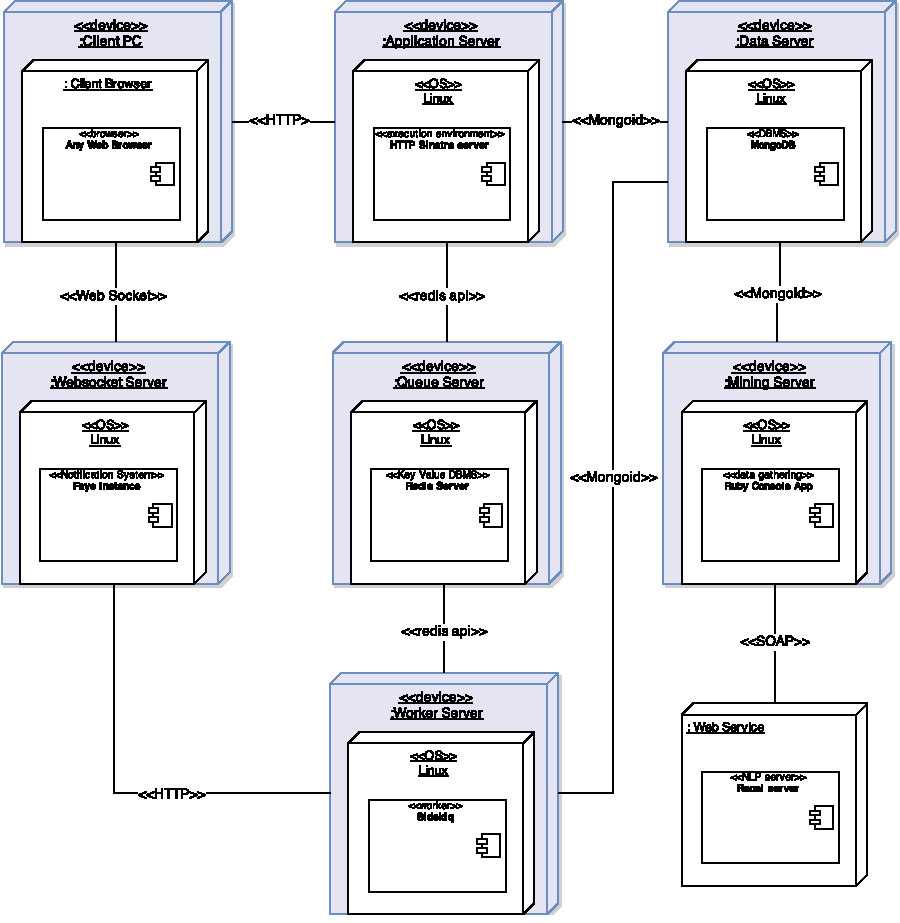
\includegraphics[width=18cm]{2_deployment}
% \caption{OpenMedia deployment diagram}\label{deployment}
% \end{figure}

% Therefore the UML diagrams concentrate on the application prototype. They cover the most useful standard diagrams: use case diagrams, sequence diagrams, class diagrams, state diagrams, activity diagrams, components diagrams and deployment diagrams. All diagrams express the relationships, structural and behavioral aspects of the system. Modeling the application is for more reasons. The first and the obvious one, is to communicate the application architecture and its behavior. But the important aspect is, while modeling the platform the problem is understood better.

% The implementation chapter focuses on the provided UML design, implements the classes and follows the use cases and sequence diagrams to define the flow of the application. The application components and dependencies will probably extend to a bigger degree. This concludes the UML description of the project, that aimed at presenting the most relevant aspect of the system and covering the general architecture of the application. The UML methodology offered a good documentation basis and a clear view on requirements of the software.